\documentclass{article}
\usepackage{tikz}
\usepackage{animate}
\usepackage{amsmath}
\usepackage{ifthen}
\usepackage{pgfmath}
\usetikzlibrary {matrix}
\usepackage{tikzlings}
\usepackage{tikzlings-penguins}
\usepackage{graphics,graphicx}

\newcommand{\token}[2]{
  \begin{scope}[yshift=-#1]
    \node [circle] at (-2,0) { $token_{#2}$};
   \node[ rectangle,fill=red] at (0,0) {};
   \node[ rectangle,fill=red!20] at (1,0) {};
   \node[ rectangle,fill=red!40] at (2,0) {};
   \node[ rectangle,fill=blue!20] at (3,0) {};
   \node[ rectangle,fill=blue!40] at (4,0) {};
   \node[ rectangle,fill=blue] at (5,0) {};
   \node[ rectangle,fill=blue!20!red] at (6,0) {};
   \node[ rectangle,fill=blue!40!red] at (7,0) {};
   \node[ rectangle,fill=blue!60!red] at (8,0) {};
   \end{scope}
}
\begin{document} 
%\begin{comment}
%\begin{tikzpicture}
%  \foreach \i in {1,2,3,4,...,8} {
%    \token{\i cm} {\i};
%}
%\end{tikzpicture}
%
%\begin{frame}[fragile,allowframebreaks]{Review of CNN} 
%  \begin{longtable}{l|l}
%  1998 &LeNet\cite{lecun1998gradient} LeCun \etal built the first deep CNN. \\ 
% 2012 &  AlexNet \cite{krizhevsky2012imagenet}pushed forward the state of the art of ImageNet classification.\\  
% 2015 &   VGGNet \cite{simonyan2015very}; GoogLeNet \cite{szegedy2015going} \cite{szegedy2016rethinking,szegedy2017inception}\\
% 2016  & ResNet \cite{he2016deep} manages to build very deep networks. \\ 
% 2017 & ResNeXt\cite{xie2017aggregated}. DenseNet\cite{huang2017densely};  MobileNet \cite{howard2017mobilenets,sandler2018mobilenetv2} \\ 
% 2018 & ShuffleNet \cite{zhang2018shufflenet,ma2018shufflenet},SENet\cite{senet}\\  
% 2019 & MnasNet \cite{tan2019mnasnet}; EfficientNet \cite{tan2019efficientnet}\\ 
% \caption{  Key milestones in the development of CNN.}
%\end{longtable}
%\end{frame}
%\end{comment}
\newcommand{\lenet} { 1998,LeNet\cite{lecun1998gradient} LeCun \etal built the first deep CNN.  } 
\newcommand{\alexnet} {2012, AlexNet \cite{krizhevsky2012imagenet}pushed forward the state of the art of ImageNet classification.  } 
\newcommand{\vggnet} { VGGNet \cite{simonyan2015very} }
\newcommand{\googlenet}{ GoogLeNet \cite{szegedy2015going} \cite{szegedy2016rethinking,szegedy2017inception} }
\newcommand{\resnet} { ResNet \cite{he2016deep} manages to build very deep networks.  } 
\newcommand{\resnext} { ResNeXt\cite{xie2017aggregated} }
\newcommand{\densenet} { DenseNet\cite{huang2017densely}}
\newcommand{\mobilenwt} {MobileNet \cite{howard2017mobilenets,sandler2018mobilenetv2} }
\newcommand{\shufflenet} { \cite{zhang2018shufflenet,ma2018shufflenet}}
\newcommand{\senet } { SENet\cite{senet}} 
\newcommand{\mnasnet} {MnasNet \cite{tan2019mnasnet}}
\newcommand{\efficientnet} {EfficientNet \cite{tan2019efficientnet}}

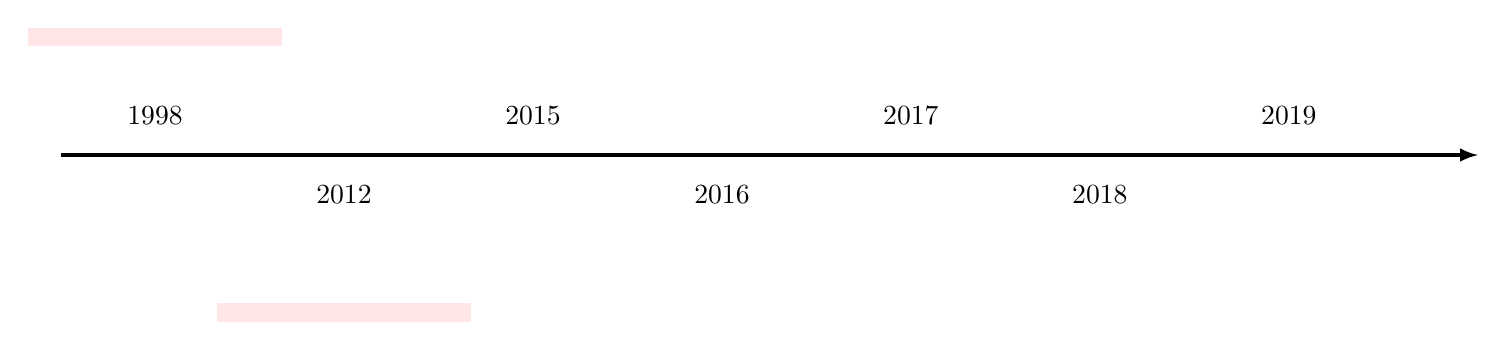
\begin{tikzpicture}[>=latex,very thick,x=1.2cm,rectangle/.style={fill=red!10,text width=3cm}] 
  \draw[->] (-2,-0.5) -- ( 13,-0.5); 
  \node  (y1998) at (-1,0) { 1998};
  \node  (y2012) at (1,-1)  {2012}; 
  \node  ( y2015) at (3,0) {2015}; 
  \node  (y2016) at ( 5,-1) {2016};
  \node  (y2017)  at (7,0) {2017};
  \node  (y2018) at (9,-1)  { 2018}; 
  \node  (y2019) at (11,0) {2019};
  \node[rectangle] (lenet)  at ( -1,1) { \lenet  } ;
  \node[rectangle] (alenet)  at (1,-2.5){ \alexnet } ;
\end{tikzpicture}


\end{document}
